\Subsection{Характеристические функции случайных величин}

\begin{definition}
    Комплекснозначная случайная величина $\xi = \Re \xi + i \Im \xi$, где $\Re \xi$ и $\Im \xi$
    вещественнозначные случайные величины.
\end{definition}

\begin{definition}
    $\xi : \Omega \to \mathbb{C}$

    $\mathbb{E} \xi = \mathbb{E} \Re \xi + i \mathbb{E} \Im \xi$
\end{definition}

\begin{properties}
    \begin{enumerate}
        \item {
            $\mathbb{E} (i \xi) = i \mathbb{E}\xi$
        }
        \item {
            Комплексная линейность $\mathbb{E} (\alpha \xi + \beta \eta) = \alpha \mathbb{E} \xi + \beta \mathbb{E} \eta$, где $\alpha, \beta \in \mathbb{C}, \xi, \eta : \Omega \to \mathbb{C}$

            \textit{Доказательство: } $\mathbb{E} (\alpha \xi) = \mathbb{E} (a + ib)\xi = \mathbb{E} (a \xi) + \mathbb{E} (b\xi i) = (a + bi) \mathbb{E} \xi$
        }
        \item {
            $\overline{\mathbb{E} \xi} = \mathbb{E} \overline{\xi}$
        }
        \item {
            $|\mathbb{E} \xi | \leqslant \mathbb{E} |\xi|$

            \textit{Доказательство: } Возьмём $c \in \mathbb{C}, |c| = 1$, такой, что $\mathbb{E} (c \xi) = |\mathbb{E} \xi|$, то есть $c = \frac{|\mathbb{E} \xi|}{\overline{\mathbb{E} \xi}}$ (или $c = e^{-i \cdot \arg \mathbb{E}\xi}$).

            Тогда $|\mathbb{E} \xi| = \mathbb{E} (c \xi) = \mathbb{E} (\Re (c \xi)) \leqslant \mathbb{E} |\Re (c \xi)| \leqslant \mathbb{E} |c \xi | = \mathbb{E} |\xi|$
        }
    \end{enumerate}
\end{properties}

\begin{definition}
    Ковариация $cov(\xi, \eta) = \mathbb{E} (\xi - \mathbb{E}\xi)\overline{(\eta - \mathbb{E} \eta)}$
\end{definition}

\begin{definition}
    Дисперсия $\mathbb{D} \xi = \mathbb{E} |\xi - \mathbb{E}\xi|^2$

    $cov(\xi, \xi) = \mathbb{D}\xi$
\end{definition}

\begin{definition}
    $\xi : \Omega \to \mathbb{R}$. Назовём характеристической функцией $\xi$:

    $\phi_\xi (t) = \mathbb{E} e^{it\xi}$, где $t \in \mathbb{R}$
\end{definition}

\begin{properties}
    \begin{enumerate}
        \item {
            $\phi_\xi (0) = 1$ и $|\phi_\xi (t)| \leqslant 1$

            \textit{Доказательство: } $|\phi_\xi (t)| \leqslant |\mathbb{E} e^{it\xi}| \leqslant \mathbb{E}|e^{it\xi}| = 1$
        }
        \item {
            $\phi_{a\xi + b} (t) = e^{ibt} \phi_\xi (at)$

            \textit{Доказательство: } $\phi_{a\xi + b} (t) = \mathbb{E} e^{i(a \xi + b)t} = \mathbb{E} e^{ibt} e^{i\xi a t} = e^{ibt} \mathbb{E} e^{i\xi (at)} = \phi_{\xi} (at) e^{ibt} $
        }
        \item {
            Если $\xi$ и $\eta$ независимы, то $\phi_{\xi + \eta} (t) = \phi_\xi (t) \cdot \phi_{\eta} (t)$

            \textit{Доказательство: } $e^{i\xi t}$ и $e^{i \eta t}$ независимы и пишем произведение матожиданий
        }
        \item {
            $\overline{\phi_{\xi}(t)} = \phi_{\xi} (-t)$

            \textit{Доказательство: } $\overline{\phi_{\xi}(t)} = \overline{\mathbb{E} e^{i \xi t}} = \mathbb{E} \overline{e^{i \xi t}} = \mathbb{E} e^{-i \xi t} = \phi_\xi (-t)$
        }
        \item {
            $\phi_{\xi}$ равномерно непрерывна на $\mathbb{R}$

            \textit{Доказательство: } $|\phi_{\xi}(t + h) - \phi_{\xi}(t)| = | \mathbb{E} e^{i (t + h) \xi} - \mathbb{E} e^{i t \xi} | = | \mathbb{E} \left( e^{it \xi} (e^{i h \xi} - 1) \right) | \leq $

            $\leq \mathbb{E} \left| e^{it \xi} (e^{i h \xi} - 1) \right| = \mathbb{E} | e^{i h \xi} - 1 | = \int_{\mathbb{R}} | e^{i h x} - 1 | d P_{\xi}(x) \rightarrow_{(*)} 0$.

            $(*)$: Знаем, что $e^{i h x} \rightarrow_{h \to 0} 1$, хотим понять, что можно вносить предел под знак интеграла. Это сделать можно по теорема Лебега, где суммируемая мажоранта будет $2$, так как мера вероятностная.

            \textbf{Напоминание Th Лебега:}\newline

            \begin{center}
                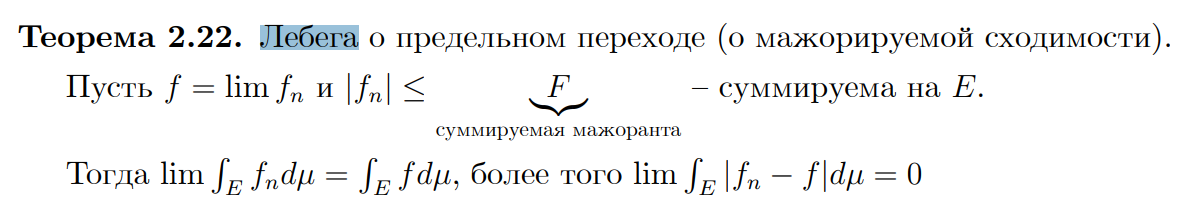
\includegraphics[scale=0.7]{./assets/03-characteristic-funcs/lebegs-theorem.PNG}
            \end{center}

            %$|\phi_{\xi} (t + h) - \phi_{\xi}(t)| = |\mathbb{E} (e^{i \xi (t + h) - \mathbb{E} e^{i \xi t}}) | = |\mathbb{E} (e^{i\xi t} \cdot e^{i \xi h}) - \mathbb{E} e^{i \xi t}| =
            %|\mathbb{E} (e^{i \xi t}(e^{i \xi h} - 1))| \leqslant \mathbb{E} |e^{i \xi t}| \cdot |e^{i \xi h} - 1| $

            %$\lim_{h \to 0} \int_{\Omega} |e^{}|$
        }
    \end{enumerate}
\end{properties}

\begin{example}
    $\xi \sim \mathcal{N}(a, \sigma^2)$. Хотим посчитать характеристическую функцию.

    Возьмём $\eta \sim \mathcal{N}(0, 1)$. Тогда $\xi = \sigma \eta + a$ - имеет нужное нам распределение.

    $\phi_{\sigma \eta + a}(t) = e^{ita} \phi_{\eta} (\sigma t)$

    Считаем для $\eta$:

    $\phi_{\eta}(t) = \mathbb{E} e^{i \eta t} = \frac{1}{\sqrt{2 \pi}} \int_{\mathbb{R}} e^{i t x} e^{-\frac{x^2}{2}} dx = \frac{1}{\sqrt{2 \pi}} e^{-\frac{t^2}{2}} \int_{\mathbb{R}} e^{- \frac{(x - it)^2}{2}} dx$.

    Посчитаем $I := \int_{\mathbb{R}} e^{-\frac{(x - it)^2}{2}} dx = \int_{-it + \mathbb{R}} e^{-\frac{z^2}{2}} dz = \int_{\Gamma_R} e^{-\frac{z^2}{2}} dz = 0$ (т.к. особых точек внутри контура нет).

    С другой стороны это также равно: $\int_{\Gamma_R} e^{-\frac{z^2}{2}} dz = \underbrace{-\int_{-R}^{R}}_{\to \sqrt{2 \pi}} + \underbrace{\int_{-R - it}^{R - it}}_{\to I} + \underbrace{\int_{R - it}^{R}}_{(*): \to 0} + \underbrace{\int_{-R}^{-R - it}}_{(*): \to 0}$


    \begin{center}
        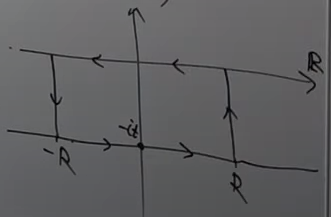
\includegraphics[width=8cm]{./assets/03-characteristic-funcs/complex-arbitrary-value-example-1.png}
    \end{center}

    $(*): \left| \int_{R - it}^{R} e^{-\frac{z^2}{2}} dz \right| =_{z = R + i y} \left| i \int_{-t}^{0} e^{- \frac{(R + iy)^2}{2}} dy \right| \leq \int_{-t}^{0} |\ldots|dy = \int_{-t}^{0} e^{\frac{-R^2 + y^2}{2}} dy \leq t e^{\frac{t^2}{2}} e^{\frac{-R^2}{2}} \rightarrow_{R \to \infty} 0$.


    Тогда получаем, что $I = \sqrt{2 \pi}$, и $\phi_{\eta}(t) = e^{-\frac{t^2}{2}}$.


    Теперь находим $\phi_{\xi}(t) = e^{iat} \phi_{\eta}(\sigma t) = e^{- \frac{\sigma^2 t^2}{2} + iat}$.
\end{example}

\begin{theorem}
    Пусть $\mathbb{E} |\xi|^n < +\infty$.

    Тогда при $k \leqslant n$ верно, что $\varphi^{(k)} (t) = \mathbb{E} ((i\xi)^k e^{i\xi t}) $.

    В частности, $\varphi^{(k)} (0) = i^k \mathbb{E} \xi^k$.

    \textit{Тут имеется в виду $k$-ая производная.}
\end{theorem}

\begin{consequence}
    Если $\mathbb{E} \xi^2 < + \infty$, то $\mathbb{E} \xi = -i \varphi'(0)$ и $\mathbb{D} \xi = -\varphi''(0) + (\varphi'(0))^2$
\end{consequence}

\begin{proof}
    Теоремы.

    Индукция по $k$

    База $k = 0$: определение $\varphi$.

    Переход $k \to k + 1$:

    $\varphi^{(k + 1)}(t) = \lim_{h \to 0} \frac{\varphi^{(k)}(t + h) - \varphi^{(k)}(t)}{h} = $

    $= \lim_{h \to 0} \frac{\mathbb{E} (i \xi)^k e^{i\xi(t + h)} - \mathbb{E} (i \xi)^k e^{it\xi}}{h} =
    \lim_{h \to 0} \mathbb{E} ((i \xi)^k e^{i t \xi} \cdot \frac{e^{ih\xi} - 1}{h}) = \mathbb{E} ((i\xi)^k e^{i t \xi} \cdot \lim_{h \to 0} \frac{e^{i h \xi} - 1}{h})$, а предел -- это $i \xi$.

    Почему можно было запихать предел под матожидание?

    $\lim \int_{\mathbb{R}} (ix)^k e^{itx} \frac{e^{ihx} - 1}{h} d P_{\xi}(x) = \int_{R} \lim_{h \to 0} ((ix)^k e^{itx} \frac{e^{ihx} - 1}{h}) d P_{\xi}(x)$ -- нужна суммируемая мажоранта.

    $\left | (ix)^k e^{itx} \frac{e^{ihx} - 1}{h}  \right | = |x|^k \left | \frac{e^{ihx} - 1}{h} \right | = (*)$.

    \begin{enumerate}
        \item {
            Если $|xh| \geqslant 1$, то $\left | \frac{e^{ihx} - 1}{h} \right | \leqslant \frac{2}{|h|} \leqslant 2|x| $ и тогда $(*) \leq 2|x|^{k + 1}$.
        }
        \item {
            Если $|xh| < 1$, то $e^{ihx} = 1 + \mathcal{O}(1 + ihx) \Rightarrow \left | \frac{e^{ihx} - 1}{h}  \right | = \left | \frac{\mathcal{O}(hx)}{h}  \right | = \mathcal{O}(x)$ и тогда $(*) = \mathcal{O}(|x|^{k + 1})$.
        }
    \end{enumerate}

    Но $\int_{\mathbb{R}} |x|^{k + 1} d P_{\xi} (x) = \mathbb{E} |\xi|^{k + 1} < +\infty$ по условию, тогда мажоранту подобрали правильную.
\end{proof}

\begin{theorem}
    Если существует $\varphi_{\xi}''(0)$ и конечна, то $\mathbb{E} \xi^2 < +\infty$
\end{theorem}

\begin{remark}
    Если существует $\varphi_{\xi}^{(2n)}$ и конечна, то $\mathbb{E} \xi^{2n} < +\infty$
\end{remark}

\begin{proof}
    $\mathbb{E} \xi^2 = \int_{\mathbb{R}} x^2 dP_{\xi} (x) = (*)$ -- хотим доказать, что этот интеграл конечен.

    Заметим, что $x = \lim_{t \to 0} \frac{\sin (tx)}{t}$ и подставим вместо $x$.

    Тогда:

    $(*) = \int_{\mathbb{R}} \lim_{t \to 0} \frac{\sin^2 (tx)}{t^2} dP_{\xi}(x) \leqslant
    \underline{\lim}_{t \to 0} \int_{\mathbb{R}} -\frac{e^{2itx} + e^{-2itx} - 2}{4t^2} dP_{\xi} (x) = (*)$ -- лемма Фату и расписали синус как $\sin{a} = \frac{e^{ia} - e^{-ia}}{2 i}$.

    $(*) = \underline{\lim}_{t \to 0} -\frac{\varphi_{\xi}(2t) - \varphi_{\xi}(-2t) - 2}{4t^2} = (*)$.

    Причём $\varphi_{\xi} (u) = \varphi_{\xi}(0) + \varphi_{\xi}'(0) \cdot u + \frac{\varphi_{\xi}''(0) u^2}{2} + o(u^2)$.

    Тогда $\varphi_{\xi}(2t) + \varphi_{\xi}(-2t) = 2 + \frac{\varphi_{\xi}''(0) \left((2t)^2 + (-2t)^2 \right)}{2} + o(t^2)$, а тогда $(*) = \underline{\lim}_{t \to 0} (-\varphi_{\xi}''(0) + o(1))$.

    То есть оценили сверху каким-то число, тогда интеграл конечен.
\end{proof}

\begin{theorem}
    \textbf{Формула обращения}

    Пусть $a < b$ и $P(\xi = a) = P(\xi = b) = 0$.

    Тогда $P(\xi \in [a, b]) = \lim_{T \to +\infty} \frac{1}{2\pi} \int_{-T}^{T} \frac{e^{-iat} - e^{-ibt}}{it} \varphi_{\xi}(t) \, dt $

    То есть $v.p. \frac{1}{2\pi} \int_{\mathbb{R}} \frac{e^{-iat} - e^{-ibt}}{it} \varphi_{\xi}(t) \, dt$
\end{theorem}

\begin{proof}

    Будем доказывать в несколько шагов:

    \begin{enumerate}
        \item {
            Пусть $\xi = \frac{b - a}{2} \eta + \frac{a +  b}{2}$, $\xi \in [a, b] \Leftrightarrow \eta \in [-1, 1]$, тогда $P(\xi \in [a, b]) = P(\eta \in [-1, 1]) = (')$.

            Допустим, что мы уже доказали эту формулу для $\eta \in [-1, 1]$, тогда

            $P(\eta \in [-1, 1]) = \lim_{T \to +\infty} \frac{1}{2\pi} \int_{-T}^{T} \frac{e^{-it} - e^{i t}}{it} \phi_{\eta}(t) dt = (*)$

            Пересчитаем левую часть формулы $(')$:

            $P(\xi \in [a, b]) = \lim_{T \to +\infty} \frac{1}{2\pi} \int_{-T}^{T} \frac{e^{i a t} - e^{i b t}}{i t} \phi_{\eta} (\frac{b - a}{2} t) e^{i \frac{a + b}{2} t} dt =_{s := \frac{b - a}{2} t}$

            $= \lim_{T \to +\infty} \frac{1}{2 \pi} \int_{-T \frac{b - a}{2}}^{T \frac{b - a}{2}} \frac{e^{i s} - e^{-i s}}{is} \phi_{\eta}(s) ds = (**)$

            То есть если мы получили, что $(*) = (**)$.

            Тогда если мы докажем формулу при $\eta \in [-1, 1]$, то решим задачу.
        }
        \item {
            Пусть $a = -1, b = 1$:

            $P(\xi \in [-1, 1]) \overset{?}{=} \lim_{T \to +\infty} \frac{1}{2\pi} \int_{-T}^{T} \frac{e^{it} - e^{-it}}{it} \phi_{\xi}(t) dt$.

            Посчитаем интеграл:

            $\int_{-T}^{T} \frac{e^{it} - e^{-it}}{it} \phi_{\xi}(t) dt = \int_{-T}^{T} \frac{e^{it} - e^{-it}}{it} \int_{\mathbb{R}} e^{itx} dP_{\xi}(x) dt =_{\text{т. Фубини}} \int_{\mathbb{R}} \int_{-T}^{T} \frac{e^{it} - e^{-it}}{it} e^{i t x} dt dP_{\xi}(x)$ -- теорему Фубини можно применять, если подъинтегральная функция суммируема: $|e^{i t x}| < 1$ и $|\frac{e^{it} - e^{-it}}{it}|$ -- ограничена (при больших $t$ значение меньше $2$, при $t \in [-1, 1]$ это непрерывная функция, а значит ограничена на этом отрезке).

            Давайте посмотрим на внутренний интеграл: $\Phi_{T}(x) = \int_{-T}^{T} \frac{e^{it} - e^{-it}}{it} e^{it x} dt$.

            Заметим, что $\frac{e^{it} - e^{-it}}{it} = \int_{-1}^{1} e^{i t u} du$.

            Тогда $\Phi_{T}(x) = \int_{-T}^{T} \int_{-1}^{1} e^{i t u} e^{i t x} du dt = \int_{-1}^{1} \int_{-T}^{T} e^{i t (u + x)} dt du$ -- т. Фубини, т.к. подъинтегральная ф-я по модулю равна $1$.


        }
    \end{enumerate}



    % $\xi = \frac{a + b}{2} + \frac{b - a}{2}\eta$, тогда $P(\xi \in [a, b]) = P(\eta \in [-1, 1])$, в частности $P_{\eta}(\{ \pm 1 \}) = 0$.

    % $\varphi_{\xi}(t) = e^{i \frac{a + b}{2} t} \varphi_{\eta}(\frac{b - a}{2}t)$ - подставим в наш интеграл.

    % $ \int_{-T}^{T} \frac{e^{-iat} - e^{-ibt}}{it} \varphi_{\xi} (t) \, dt = \int_{-T}^{T} \frac{e^{-iat} - e^{-ibt}}{it} e^{i \frac{a + b}{2} t} \varphi_{\eta} (\frac{b - a}{2} t) \, dt = $

    % $ = \int_{-T}^{T} \frac{e^{-i\frac{a - b}{2}t} - e^{-i\frac{b - a}{2}t}}{it} \varphi_{\eta} (\frac{b - a}{2}) \, dt = \int_{-\frac{b - a}{2}T}^{\frac{b - a}{2}T} \frac{e^{is} - e^{-is}}{is} \varphi_{\eta} (s) \, ds$, здесь замена $s = \frac{b - a}{2} t$

    % Можно считать, что $a = -1$, а $b = 1$

    % $\int_{-T}^T \frac{e^{it} - e^{-it}}{it} \varphi_{\xi}(t) \, dt = \int_{-T}^T \int_{\mathbb{R}} \frac{e^{it} - e^{-it}}{it} e^{itx} dP_{\xi}(x) \, dt = (*)$ - давайте переставим местами интегралы.

    % Нужна суммируемость того, что под интегралом, а она есть, всё ограничено какой-то суммируемой константой.

    % $(*) = \int_{\mathbb{R}} \int_{-T}^T \frac{e^{it} - e^{-it}}{it} e^{itx} \, dt \, dP_{\xi}(x)$.  Пусть $\Phi_T (x) = \int_{-T}^{T} \frac{e^{it} - e^{-it}}{it} e^{itx} \, dt$

    % $\lim_{T \to +\infty} \int_{-T}^T \frac{e^{it} - e^{-it}}{it} \varphi_{\xi} (t) \, dt = \lim_{T \to +\infty} \int_{\mathbb{R}} \Phi_T(x) dP_{\xi} (x) = \int_{\mathbb{R}} \lim_{T \to +\infty} \Phi_T (x) \, dP_{\xi} (x) $ - хотим понять, почему
    % можно внести предел под интеграл, но разберемся с этим позже.

    % $\lim_{T \to +\infty} \Phi_T (x) = \lim_{T \to +\infty} \int_{-1}^1 \int_{-T}^T e^{it(u + x)} \, dt \, du = (*)$.

    % Заметим, что $\frac{e^{it(u + x)}}{i(u + x)} \bigg |_{t = -T}^{t = +T} = \frac{2\sin ((u + x)T)}{u + x}$ -- первообразная для внутреннего интергала $(*)$.

    % Тогда $(*) = \lim_{T \to +\infty} \int_{-1}^1 \frac{2\sin ((u + x)T)}{u + x} \, du = (*)$. Сделаем замену $y = (u + x)T$, тогда $dy = T \cdot du$.

    % Тогда $(*) = \lim_{T \to +\infty} \int_{(-1 + x)T}^{(1 + x)T} \frac{2 \sin y}{y} \, dy = \begin{cases}
    %     0, & \text{при $x > 1$} \\
    %     0, & \text{при x < -1} \\
    %     \int_{\mathbb{R}} \frac{2 \sin y}{y} \, dy = 2\pi, & \text{иначе}
    % \end{cases}$

    % Получили $2\pi \int_{\mathbb{R}} \mathds{1}_{[-1, 1]} (x) \, dP_{\xi} (x) = 2\pi P_{\xi}([-1, 1])$.

    % Вспомним, что мы не доказали по дороге один переход. Нужно понять, почему $\int_{a}^b \frac{\sin y}{y} \, dy$ ограничен - интеграл по лучу сходится, значит первообразная
    % в бесконечностях имеет предел, значит в середине тоже ограничена, потому что непрервность - обоснование примерно такое.


    $\lim_{T \to +\infty} \Phi_T (x) = \lim_{T \to +\infty} \int_{-1}^1 \int_{-T}^T e^{it(u + x)} \, dt \, du = (*)$.

    Заметим, что $\frac{e^{it(u + x)}}{i(u + x)} \bigg |_{t = -T}^{t = +T} = \frac{2\sin ((u + x)T)}{u + x}$ -- первообразная для внутреннего интергала $(*)$.

    Тогда $(*) = \lim_{T \to +\infty} \int_{-1}^1 \frac{2\sin ((u + x)T)}{u + x} \, du = (*)$. Сделаем замену $y = (u + x)T$, тогда $dy = T \cdot du$.

    Тогда $(*) = \lim_{T \to +\infty} \int_{(-1 + x)T}^{(1 + x)T} \frac{2 \sin y}{y} \, dy = \begin{cases}
        0, & \text{при $x > 1$} \\
        0, & \text{при x < -1} \\
        \int_{\mathbb{R}} \frac{2 \sin y}{y} \, dy = 2\pi, & \text{иначе}
    \end{cases}$

    Получили, что $\lim_{T \to \infty} \Phi_T(x) = 2 \pi \cdot \mathds{1}_{[-1, 1]} (x)$.

    Если докажем, что $\int_{\mathbb{R}} \Phi_{T} (x) d P_{\xi}(x) \underbrace{\to_{\text{почти везде}}}_{\text{пользуемся } P(\xi = a) = P(\xi = b) = 0 } \int_{\mathbb{R}} 2 \pi \cdot \mathds{1}_{[-1, 1]} (x) d P_{\xi}(x)$, то решим задачу, т.к. правая часть это как раз $2 \pi P(\xi \in [-1, 1])$.

    То есть нужно понять, почему $\int_{a}^b \frac{\sin y}{y} \, dy$ ограничен -- интеграл по лучу сходится, значит первообразная в бесконечностях имеет предел, значит в середине тоже ограничена, потому что непрервность -- обоснование примерно такое.

\end{proof}

\begin{consequence}
    \begin{enumerate}
        \item {
            Если $\varphi_{\xi}(t) = \varphi_{\eta}(t)$, то $P_{\xi} = P_\eta$

            \textit{Доказательство: } Рассмотрим $A = \{ a \in \mathbb{R} \, : \, \text{$a$ - точка непрервности функции распределения} \}$.

            Тогда $\mathbb{R} \setminus A$ - не более чем счётное.
            Если $a < b$ и $a, b \in A$, то $P_{\xi} ([a, b]) = P_\eta ([a, b])$

            \begin{enumerate}
                \item {
                    Пусть $a \in \mathbb{R}, b \in A$:

                    Рассмотрим $a_n \in A$, такие, что $a_n \to a$ и убывают.

                    $P_{\xi} ((a, b]) = \lim_{n \to \infty} P_{\xi} ([a_n, b_n]) = \lim P_{\eta} ([a_n, b_n]) = P_\eta ((a, b])$.
                }
                \item {
                    Пусть $a < b$ произвольные:

                    Возьмём $b_n \in A$, такие, что $b_n \to b$ и убывают. Тогда $P_{\xi} ((a, b]) = \lim_{n \to \infty} P_{\xi} (a, b_n] = \lim P_\eta (a, b_n] = P_\eta (a, b] \Rightarrow
                    P_\xi = P_\eta$ на ячейках, а тогда по единственности продолжения везде совпадают.
                }
            \end{enumerate}
        }

        \item {
            Если $\int_{\mathbb{R}} |\varphi_\xi (t) | \, dt < +\infty$, то $\xi$ имеет плотность распределения
            $p_{\xi} (x) = \frac{1}{2\pi} \int_{\mathbb{R}} e^{-itx} \varphi_{\xi} (t) \, dt$ - преобразование Фурье.

            \textit{Доказательство: } Из суммируемости $\varphi_\xi (t) \Rightarrow P_{\xi} ((a, b]) = \frac{1}{2\pi} \int_{-\infty}^{+\infty} \frac{e^{-iat} - e^{-ibt}}{it} \varphi_{\xi} (t) \, dt$.

            Проверим, что $P_{\xi} (a, b] = \int_a^b p_{\xi} (x) \, dx$.

            $\int_a^b p_{\xi} (x) \, dx = \frac{1}{2\pi} \int_a^b \int_{\mathbb{R}} e^{-itx} \varphi_\xi (t) \, dt \, dx = (*)$. Под внутренним интегралом суммируемая функция, значит можно переставлять местми интегралы.

            Тогда $(*) = \frac{1}{2\pi} \int_{\mathbb{R}} \int_a^b e^{-itx} \, dx \varphi_\xi (t) \, dt$
        }
    \end{enumerate}
\end{consequence}

\begin{theorem}
    $\xi_k \sim \mathcal{N} (a_k, \sigma_k^2)$, $c_k \in \mathbb{R}$ не все нулевые и $\xi_k$ -- независимы и $\xi = a_0 + \sum_{k = 1}^n c_k \xi_k$.

    Тогда $\xi \sim \mathcal{N} (a, \sigma^2)$, где
    $a = a_0 + \sum_{k = 1}^n c_k a_k$ и $\sigma^2 = \sum_{k = 1}^n c_k^2 \sigma_k^2$.
\end{theorem}

\begin{proof}
    $\varphi_{\xi} (t) = \varphi_{a_0} (t) \varphi_{c_1\xi_1} (t) \ldots \varphi_{c_n\xi_n} (t) = $

    $=  e^{ita_0} (t) \varphi_{\xi_1} (c_1t) \ldots \varphi_{\xi_n} (c_nt) =
    e^{ita_0} e^{ia_1c_1 t} e^{- \frac{(c_1 \sigma_1 t)^2}{2}} \ldots e^{ia_nc_n t} e^{- \frac{(c_n \sigma_n t)^2}{2}} =
    e^{ita} e^{- \frac{\sigma^2t^2}{2}} $
\end{proof}

\Subsection{Сходимость по распределению}

\begin{remark}
    \begin{enumerate}
        \item {
            Точек, где нет непрерывности $F_{\xi}$ не более чем счётное множество

            %\begin{proof}
            %    $P(\xi = x) > 0$ - эти точки, а мера вероятностная.
            %\end{proof}
        }
        \item {
            Если $F_{\xi_n}(b) - F_{\xi_n} (a) \rightarrow F_{\xi}(b) - F_{\xi}(a)$ для всех $a, b$, за исключением счётного множества.

            Тогда $F_{\xi_n}(b) \rightarrow F_{\xi} (b)$ за исключением счётного множества.

            \begin{proof}
                Рассмотрим $F(x)$, функцию распределения. Возьмём хорошие $a$, т.ч. $F(a) < \varepsilon$ и
                $b$, т.ч. $F(b) > 1 - \varepsilon$.

                Тогда $(F_n(b) - F_n (a)) - (F(b) - F(a)) \rightarrow 0 \implies
                |(F_n(b) - F_n(a)) - \underbrace{(F(b) - F(a))}_{> 1 - 2\varepsilon}| < \varepsilon \implies F_n(b) - F_n(a) > 1 - 3\varepsilon \implies F_n(a) < 3\varepsilon$ при больших $n$.

                Возьмём хорошее $x$, $|F_n(x) - F(x)| \leqslant |(F_n(x) - F_n(a)) - (F(x) - F(a))| + \underbrace{F_n(a)}_{<3\varepsilon} + \underbrace{F(a)}_{<\varepsilon} < 5\varepsilon$ при больших $n$
            \end{proof}
        }
        \item {
            $D \subset \mathbb{R}$ не более чем счётное и $U \subset \mathbb{R}$ - открытое.

            Тогда $U = \bigcup_{k = 1}^{\infty} (a_k, B_k]$, где $a_k, b_k \not \in D$

            \begin{proof}
                Нарезаем открытое множество с шагом 1, тем ячейки, которые целиком попали - берём. Те, что не попали - бьём пополам и так далее.
            \end{proof}
        }
        \item {
            $\xi$ и $\eta$ независимые и $\eta$ имеет непрерывное распределение.

            Тогда $\xi + \eta$ имеет непрерывное распределение.

            \begin{proof}
                $P_{\xi + \eta} = P_{\xi} * P_{\eta}$

                $P_{\xi + \eta} (\{ a \}) = \int_{\mathbb{R}} \underbrace{P_{\eta} ( \{ a - x \} )}_{= 0, \text{т.к. непрерывность}}  dP_{\xi} (x) $
            \end{proof}
        }
    \end{enumerate}
\end{remark}

\begin{definition}
    Множество $B \subset \mathbb{R}$ - регулярное, относительно $P_{\xi}$, если $P_{\xi} (Cl \, B \setminus Int \, B) = 0$,
    то есть $P(\xi \in Cl \, B \setminus Int \, B) = 0$
\end{definition}

\begin{theorem}
    $\xi, \xi_1, \xi_2, \ldots$ - случаный величины, $F, F_1, F_2, \ldots$ - их функции распределения, а
    $\varphi, \varphi_1, \varphi_2, \ldots$ - их характеристичечкие функции. Следующие условия равносильны:

    \begin{enumerate}
        \item $\xi_n$ сходится к $\xi$ по распределению
        \item Для любого $U$ открытого $\underline{\lim} P(\xi_n \in U) \geqslant P(\xi \in U)$
        \item Для любого $A$ замкнутого $\overline{\lim} P(\xi_n \in A) \leqslant P(\xi \in A)$
        \item Для любого $B$ регулярного борелевского $\lim P(\xi_n \in B) = P(\xi \in B)$
        \item Для любого $B$ регулярного борелевского $\lim \mathbb{E} \mathds{1}_{B}(\xi_n) = \mathbb{E} \mathds{1}_B (\xi)$
        \item Для любой $f$ непрерывной на прямой и ограниченной $\lim \mathbb{E} f(\xi_n) = \mathbb{E} f(\xi)$
        \item $\varphi_n$ сходится к $\varphi$ поточечно
    \end{enumerate}
\end{theorem}

\begin{proof}
    \begin{enumerate}
        \item {
            $2 \Longleftrightarrow 3$

            Если $A = \mathbb{R} \setminus U$, тогда $P(\xi_n \in A) = 1 - P(\xi_n \in U)$.

            $P(\xi \in A) > \overline{\lim} P(\xi_n \in A) = 1 - \underline{\lim} P(\xi_n \in U) \leqslant 1 - P(\xi \in U) = P(\xi \in A)$
        }
        \item {
            $2 \cup 3 \implies 4$

            Мы знаем, что $U = \{ \xi_n \in Int \, B \} \{ \xi_n \in B \} \subset \{ \xi_n \in Cl \, B \} = A$

            Тогда $P(\xi_n \in U) \leqslant P(\xi_n \in B) \leqslant P(\xi_n \in A) \implies \underbrace{\overline{\lim} P(\xi_n \in B)}_{\geqslant \underline{\lim} P(\xi_n \in B) \geqslant \underline{\lim} P(\xi_n \in U) \geqslant P(\xi \in U) = P(\xi \in B)} \leqslant \overline{\lim} P(\xi_n \in A) \leqslant P(\xi \in A) = P(\xi \in B)$
        }
        \item {
            $4 \Longleftrightarrow 5$

            $\mathbb{E} \mathds{1}_B (\xi_n) = P(\mathds{1}_B (\xi_n) = 1) = P(\xi_n \in B)$
        }
        \item {
            $6 \implies 7$

            $\varphi_{\eta} (t) = \mathbb{E} e^{et\eta} = \mathbb{E} \cos (t\eta) + i \mathbb{E} \sin (t \eta)$

            Тогда $\varphi_n(t) = \mathbb{E} \cos (t \xi_n) + i\mathbb{E} \sin (t\xi_n) \rightarrow \mathbb{E} \cos (t\xi) + i \mathbb{E} \sin (t\xi) = \varphi (t)$
        }
        \item {
            $1 \implies 2$

            Берём открытое $U$, по замечанию $U =  \bigcup\limits_{k = 1}^{\infty} (a_k, b_k]$, где $a_k, b_k$ - точки непрерывности $F$.

            $\{ \xi_n \in U \} \supset \{ \xi_n \in \bigcup\limits_{k = 1}^{m} (a_k, b_k] \} \implies P(\xi_n \in U) \geqslant \sum_{k = 1}^m P(\xi_n \in (a_k, b_k])$

            $\underline{\lim} P(\xi_n \in U) \geqslant \underline{\lim} \sum_{k  = 1}^m \geqslant \sum_{k = 1}^m \underline{\lim} P(\xi_n \in (a_k, b_k]) \overset{*}{=} \sum_{k = 1}^m P(\xi \in (a_k b_k]) \overset{m \to \infty}{\rightarrow} \sum_{k = 1}^{\infty} P(\xi \in (a_k, b_k]) = P(\xi \in U)$

            А значит $\underline{\lim} P(\xi_n \in U) \geqslant P(\xi \in U)$

            $(*) P(\xi_n \in (a_k, b_k]) = F_n (b_k) - F_n (a_k) \rightarrow F(b_k) - F(a_k) = P(\xi \in (a_k, b_k])$
        }
        \item {
            $5 \implies 6$

            Пусть $|f| \leqslant M$ и $D = \{ x \in \mathbb{R} \, : \, P(f(\xi) = x) > 0 \} = \{ x \, : \, P_{\xi} (f^{-1} (x) > 0) \}$. Это не более чем счётное множество. Потому что для разных $x$ - это дизъюнктные.
            Множеств с вероятностью $\frac{1}{2}$ - не больше двух, с вероятностью $\frac{1}{3}$ не больше трёх и так далее.

            Пусть $-M = t_0 < t_1 < \ldots < t_m = M$, так, что $t_y \not \in D$ и мелкость $< \varepsilon$.

            Заведём множества $A_j = \{ x \in \mathbb{R} \, : \, t_{j - 1} \leqslant f(x) \leqslant t_j \} \supset B_j = \{ x \in \mathbb{R} \, : \, t_{j - 1} < f(x) \leqslant t_j \} \supset U_j = \{ x \in \mathbb{R} \, : \, t_{j - 1} < f(x) < t_j \}$. Где $A_j$ - замкнутое,а $U_j$ - открытое.

            Мы поняли, что $U_j \subset Int \, B_j \subset B_j \subset Cl \, B_j \subset A_j \implies Cl \, B_j \setminus Int \, B_j \subset A_j \setminus U_j$

            Тогда $B_j$ регулярно относительно $P_\xi$

            Определим $g(x) = \sum_{j = 1}^{m} t_{j - 1} \mathds{1}_{B_j} (x)$. Тогда $g(x) < f(x) < g(x) + \varepsilon$.

            $|g(x) - f(x)| < \varepsilon$ и тогда $\mathbb{E} |g(\xi_n) - f(\xi_n)| \leqslant \varepsilon$ и мы знаем, что $\mathbb{E}g(\xi_n) \rightarrow \mathbb{E}g(\xi)$ - видно, если расписать матожидание $g$ по линейности.

            $\mathbb{E} |f(\xi_n) - f(\xi)| \leqslant |\mathbb{E} f(\xi_n) - \mathbb{E} g(\xi_n)| + |\mathbb{E} g(\xi_n) - \mathbb{E} g(\xi)| + |\mathbb{E} g(\xi) - \mathbb{E} f(\xi) | < 3\varepsilon$ при больших $n$, каждый из модулей $< \varepsilon$
        }
        \item {
            $7 \implies 1$

            Возьмём $\eta \sim \mathcal{N} (0, \sigma^2)$, такую, что $\eta$ не зависит от всех $\xi_n$ и $\xi$

            $\varphi_{\xi_n + \eta} (t) = \varphi_{\xi_n} (t) \varphi_{\eta} (t) = \varphi_{n} (t) \cdot e^{-\frac{\sigma^2 t^2}{2}} \overset{\text{поточечно}}{\rightarrow} \varphi(t) e^{-\frac{\sigma^2t^2}{2}} = \varphi_{\xi + \eta} (t)$

            $\xi_n + \eta$ и $\xi + \eta$ имеют непрерывное распределение, поэтому можем не задумываясь писать формулу обращения:

            $P(\xi_n + \eta \in (a, b]) = \frac{1}{2\pi} \int_{\mathbb{R}} \frac{e^{-iat} - e^{-ibt}}{it} \varphi_{\xi_n + \eta} (t) \, dt \overset{*}{\rightarrow} \frac{1}{2\pi} \int_{\mathbb{R}} \frac{e^{-iat} - e^{-ibt}}{it} \varphi_{\xi + \eta} \, dt = P(\xi + \eta \in (a, b])$.

            $(*)$ Нужна суммируемая мажоранта $\left | \frac{e^{-iat} - e^{-ibt}}{it} \varphi_{\xi_n + \eta} (t) \right | \leqslant e^{-\frac{\sigma^2t^2}{2}}$ - суммируемая мажоранта.

            То есть $\underbrace{P(\xi_n + \eta \in (a, b])}_{G_n (b) - G_n(a)} \rightarrow \underbrace{P(\xi + \eta \in (a, b])}_{G(b) - G(a)}$, где $G_n (x) = F_{\xi_n + \eta}(x)$ и $G(x) = F_{\xi + \eta} (x)$

            Тогда из замечания $G_n(x) \rightarrow G(x)$

            Возьмём $x$ - точка непрерывности $F$ и выберем $\delta > 0$, так, что $|F(x \pm \delta) - F(x)| < \varepsilon$ - есть из непрерывности.

            $ \{ \xi_n + \eta \leqslant x - \delta \} \setminus \{ |\eta| > \delta \} \subset  \{ \xi_n \leqslant x \} \subset \{ \xi_n + \eta \leqslant x + \delta \} \cup \{ |\eta| > \delta \}$.

            Тогда $\underbrace{G_{n} (x - \delta) - P(|\eta| > \delta)}_{G_n (x - \delta - \frac{\sigma^2}{\delta^2}) > G_n (x - \delta) - \varepsilon > G(x - \delta) - 2\varepsilon > F(x - 2\delta) - 3\varepsilon > F(x) - 4\varepsilon} \leqslant F_n (x) \leqslant
            \underbrace{G_{n} (x + \delta) + P(|\eta| > \delta)}_{G_n (x + \delta) + \frac{\sigma^2}{\delta^2} < G_n (x + \delta) + \varepsilon < G(x + \delta) + 2\varepsilon < F(x + 2\delta) + 3\varepsilon < F(x) + 4\varepsilon}$

            Оценим вероятность: $P(|\eta| > \delta) \leqslant \frac{\mathbb{D} \eta}{\delta^2} = \frac{\sigma^2}{\delta^2}$


        }
    \end{enumerate}
\end{proof}

\begin{theorem}
    $F_n, F \, \mathbb{R} \to [0, 1]$ монотонные, $F \in C(\mathbb{R})$ и
    $F_n \to F$ поточечно.

    Тогда $F_n \rightrightarrows F$
\end{theorem}

\begin{proof}
    Берём $\varepsilon > 0$ и $m > \frac{1}{\varepsilon}$. Пусть $t_j$, такие, что $F(t_j) = \frac{j}{m}$. Если для большого $j$ точки не нашлось, то
    $F < \frac{j + 1}{m}$, а если для маленького не нашлось, то $F > \frac{j - 1}{m}$ (потому что иначе из непрерывности такие точки найдутся).

    Знаем, что $F_n(t_j) \rightarrow F(t_j)$. Берём $N \, : \, \forall \, n \geqslant N \, |F_n(t_j) - F(t_j)| < \varepsilon$.

    Теперь смотрим на произвольную точку: $t_j < t < t_{j + 1}$. Тогда
    $F_n(t) \leqslant F_n(t_{j + 1}) < F(t_{j + 1}) + \varepsilon = \frac{j + 1}{m} + \varepsilon = F(t_j) + \frac{1}{m} + \varepsilon \leqslant F(t) + \frac{1}{m} + \varepsilon < F(t) + 2\varepsilon$.

    Аналогично в другую сторону:

    $F_n (t_j) > F(t_j) - \varepsilon = \frac{j}{m} - \varepsilon = F(t_{j + 1}) - \frac{1}{m} - \varepsilon \geqslant F(t) - 2\varepsilon$.

\end{proof}

\Subsection{Центральная предельная теорема}

\begin{theorem}
    \textbf{ЦПТ в форме Леви}

    $\xi_1, \xi_2, \ldots $ независимые, одинаково распределённые случайные величины. $a = \mathbb{E} \xi_1,
    \sigma^2 = \mathbb{D} \xi_1, S_n = \xi_1 + \xi_2 + \ldots + \xi_n$.

    Тогда $P \left ( \frac{S_n - nq}{\sigma \sqrt{n}} \leqslant x \right ) = P\left ( \frac{S_n - \mathbb{E} S_n}{\sqrt{\mathbb{D} S_n}} \leqslant x \right ) \rightrightarrows \Phi (x) = \frac{1}{\sqrt{2\pi}} \int_{-\infty}^x e^{-\frac{t^2}{2}} \, dt$
\end{theorem}

\begin{proof}
    Достаточно проверять поточечную сходимость характеристических функций.

    $\varphi_{\xi_k - a} (t) = 1 - \frac{\sigma^2 t^2}{2} + o(t^2)$, потому что
    мы знаем, что $\mathbb{E} (\xi_k - a) = 0$ и $\mathbb{D} (\xi_k - a) \sigma^2$

    Тогда $\varphi_{S_n - na} (t) = \prod\limits_{k = 1}^n \varphi_{\xi_k - a} (t) = \left ( 1 - \frac{\sigma^2t^2}{2} + o(t^2) \right )^n$

    $\varphi_{\frac{S_n - na}{\sigma \sqrt{n}}} = \varphi_{S_n - na} \left ( \frac{t}{\sqrt{n}\sigma} \right ) = \left( 1 - \frac{t^2}{2n} + o(\frac{t^2}{n}) \right) \rightarrow e^{-\frac{t^2}{2}}$.

    Чтобы получить последний переход - логарифмируем.

    То есть $\frac{S_n - na}{\sqrt{n} \sigma}$ сходится по распределению к $\mathcal{N} (0, 1) \implies$ функция распределения сходится равномерно.
\end{proof}

\begin{consequence}
    \textbf{Интегральная теорема Муавра-Лапласа}

    $S_n$ - количество успехов в схеме Бернулли с вероятностью успеха $p \in (0, 1)$.

    Тогда $P \left( \frac{S_n - np}{\sqrt{npq}} \leqslant \right) \rightrightarrows \Phi (x)$
\end{consequence}

\begin{proof}
    $\mathbb{E} \xi_k = p, \mathbb{D} \xi_k = pq$
\end{proof}

\begin{example}
    \textbf{Посчитаем характеристическую функцию для Poisson($\lambda$)}

    $\varphi_{\xi} (t) = \mathbb{E} e^{i t \xi} = \sum_{n = 0}^\infty e^{itn} \frac{e^-\lambda \lambda^n}{n!} = \sum_{n = 0}^\infty \frac{(\lambda e^{it})^n}{n!} \cdot e^{-\lambda} = exp (\lambda (e^{it} - 1))$
\end{example}

\begin{theorem}
    $P(\xi_{nk} = 1) = p_{nk}$ и $P(\xi_{nk} = 0) = 1 - p_{nk}$ и пусть $S_n = \xi_{n1} + \ldots + \xi_{nn}$.

    $\max \{ p_{n1}, \ldots, p_{nn} \} \rightarrow 0$ и $p_{n1} + \ldots p_{nn} \rightarrow \lambda$.

    Тогда $P(S_n = k) \rightarrow \frac{\lambda^k e^{-\lambda}}{k!}$
\end{theorem}

\begin{proof}
    $\varphi_{\xi_{nk}} (t) = \mathbb{E} e^{it\xi_{nk}} = 1 - p_{nk} + p_{nk}e^{it} = 1 + p_{nk} (e^{it} - 1)$

    Тогда $\varphi_{S_n} = \prod_{k = 1}^n (1 + p_{nk} (e^{it} - 1)) \overset{?}{\rightarrow} exp (\lambda (e^{it} - 1)) $.

    Пусть $z = e^{it} - 1$

    Значит, нужно проверить $\sum_{k = 1}^n \ln (1 + p_{nk} z) \rightarrow \lambda z$. Раскладываем логарифм:

    $\underbrace{\sum_{k = 1}^n p_{nk} z}_{\rightarrow \lambda z} + \sum_{k = 1}^n \mathcal{O} (p_{nk}^2)$. Значит осталось показать, что вторая сумма стремится к нулю.

    Действительно, $\sum_{k = 1}^n \mathcal{O} (p_{nk}^2) \leqslant (p_{n1} + \ldots p_{nn}) \cdot \max \{ p_{n1}, \ldots, p_{nn} \}  \rightarrow 0$
\end{proof}

\begin{theorem}
    \textbf{ЦПТ в форме Линденберга}

    $\xi_1, \ldots$ - независимые случайные величины, $a_k = \mathbb{E} \xi_k, \sigma_k^2 = \mathbb{D} \xi_k > 0, S_n = \xi_1 + \ldots + \xi_n, \mathbb{D}_n^2 = \sum_{k = 1}^n \sigma_k^2$

    $f(x) = x^2 \mathds{1}_{\{ |x| \geqslant \varepsilon \mathbb{D}_n \} } (x) \, \forall \, \varepsilon > 0$ и $Lind (\varepsilon, n) = \frac{1}{\mathbb{D}_n^2} \sum_{k = 1}^n \mathbb{E} f (\xi_k - a_k) \rightarrow 0$

    Тогда $P \left( \frac{S_n - \mathbb{E} S_n}{\sqrt{\mathbb{D} S_n}} \leqslant x \right) \rightrightarrows \Phi (x)$
\end{theorem}

\begin{theorem}
    \textbf{ЦПТ в форме Ляпунова}

    $\xi_1, \ldots$ независимые случайные величины

    $L(\delta, n) = \frac{1}{\mathbb{D}_n^{2 + \delta}} \sum_{k = 1}^n \mathbb{E} | \xi_k - a_k |^{2 + \delta} \rightarrow 0$ при некотором $\delta$

    Тогда $P\left( \frac{S_n - \mathbb{E} S_n}{\sqrt{\mathbb{D} S_n}} \leqslant x \right) \rightrightarrows \Phi (x)$
\end{theorem}

\begin{proof}
    %Ляпунов из Линденберга:
    % TODO
    %$Lind (\varepsilon, n) = \frac{1}{\mathbb{D}_n^2} \sum_{k = 1}^n \mathbb{E} (|\xi_k - a_k|^2 \cdot \mathds{1}_{|x| \geqslant \varepsilon \mathbb{D}_n} (\xi_k - a_k) ) \leqslant \frac{1}{\mathbb{D}_n^2} \sum_{k = 1}^n \mathbb{E} \left( \frac{|\xi_k - a_k|^{2 + \delta}}{} \right)$
\end{proof}

\begin{theorem}
    Пусть $\delta \in [0, 1]$ и $\xi_1, \ldots$ независимые случаные величины.

    Тогда $\left | P \left( \frac{S_n - \mathbb{E} S_n}{\sqrt{\mathbb{D} S_n}} \leqslant x \right) - \Phi (x) \right | \leqslant C_{\delta} L (\delta, n)$
\end{theorem}

\begin{theorem}
    \textbf{Берри-Эссенна}

    $\xi_1, \ldots$ независимые, одинаково распределённые случаные величины.

    Тогда$\left | P \left( \frac{S_n - na}{\sqrt{\sqrt{n} \sigma}} \leqslant x \right) - \Phi (x) \right | \leqslant C_{\delta} \cdot \frac{\mathbb{E} |\xi_1 - a|^{2 + \delta}}{n^{\frac{\delta}{2}} \sigma^{2 + \delta}}$
\end{theorem}

\begin{proof}
    $\mathbb{D}_n^2 = n \sigma^2$ и $L (\delta, n) = \frac{1}{n^{1 + \frac{\delta}{2} \cdot \sigma^{2 + \delta}}} \cdot n \mathbb{E} |\xi_1 - a|^{2 + \delta}$

    В частности при $\delta = 1 \, |P - \Phi| \leqslant C \frac{\mathbb{E} |\xi_1 - a|^3}{\sqrt{n} \sigma^3}$
\end{proof}

\begin{remark}
    \textbf{Про константы}

    \begin{enumerate}
        \item {
            Эссен (1956) $C \geqslant \frac{3 + \sqrt{10}}{6 \sqrt{2 \pi}} \approx 0,4097$
        }
        \item {
            Шевцова (2014) $C \leqslant 0,469$
        }
        \item {
            Для общего случая: $C_1 \leqslant 0,5583$
        }
        \item {
            Для схемы Бернулли (2018) $C_1 \leqslant 0,4099$
        }
        \item {
            Для схемы Бернулли с $p = \frac{1}{2}$ $C = \frac{1}{\sqrt{2\pi}}$
        }
    \end{enumerate}
\end{remark}

\begin{theorem}
    \textbf{Хартмана-Винтнера (закон повторного логарифма)}

    $\xi_1, \xi_2, \ldots$ - независимые, одинаково распределённые. $\mathbb{E} \xi_1 = 0, \, \mathbb{D} \xi_1 = \sigma^2 > 0$

    Тогда $\overline{\lim} \frac{S_n}{\sqrt{2n \ln \ln n}} = \sigma$, а $\underline{\lim} \frac{S_n}{\sqrt{2n \ln \ln n}} = -\sigma$
\end{theorem}

\begin{theorem}
    \textbf{Штрассена}

    $\xi_1, \xi_2 \ldots$ независимые одинаково распределённые, $\mathbb{E} \xi_1 = 0$ и $\mathbb{D} \xi_1 = \sigma^2 > 0$

    Тогда любое число из $[-\sigma, \sigma]$ - пред. точка послед. $\frac{S_n}{\sqrt{2n \ln \ln n}}$
\end{theorem}


\Subsection{Большие уклонения}

 \textbf{ЗБЧ в форме Чебышёва}

 $\xi_1, \xi_2, \ldots$ - незаисимые, одинаково распределённые случайные величины. $\mathbb{E} \xi_1 = a, \mathbb{D} = \sigma^2 > 0$

 Тогда $P\left(\frac{S_n}{n} \geqslant r \right) \rightarrow 0$, если $r > a$

 Более того, $P \left( \frac{S_n}{n} \geqslant r \right) \leqslant \frac{\sigma^2}{(r - a)n}$ - это оценка из доказательства. Но оценка довольно плохая.

 \begin{definition}
    $\xi$ удовлетворяет условию Крамера, если при $\lambda \in (0, \lambda_0)\, : \, \mathbb{E} e^{\lambda \xi} < +\infty$
 \end{definition}

 \begin{theorem}

    \textbf{Оценка Чернова}

    $\xi_1, \xi_2, \ldots$ - независимые, одинаково распределённые, удовлетворяющие условию Крамера и $r > a = \mathbb{E}\xi_1$

    Хотим оценить $P\left( \frac{S_n}{n} \geqslant r \right) = P\left( S_n \geqslant nr \right) = P\left( \lambda S_n \geqslant \lambda nr \right) = P\left( e^{ \lambda S_n} \geqslant e^{\lambda nr} \right) \overset{\text{Марков}}{\leqslant} \frac{\mathbb{E} e^{\lambda S_n}}{e^{\lambda n r}}
    \overset{*}{=} \left( \frac{\mathbb{E} e^{\lambda \xi_1}}{e^{\lambda r}}  \right)^n$

    $(*) \mathbb{E} e^{\lambda S_n} = \mathbb{E} (\prod_{k = 1}^n e^{\lambda \xi_k}) = (\mathbb{E} e^{\lambda \xi_1})^n$

    А теперь, то что получилось - будем минимизировать по $\lambda$

    $\varphi (\lambda) = \ln \mathbb{E} e^{\lambda \xi_1} - \lambda r \rightarrow \inf$, где $\lambda$ допустимое

    $I(r) = \sup_{\lambda} \{ \lambda r - \ln (\mathbb{E} e^{\lambda \xi_1}) \} \implies P \left( \frac{S_n}{n} \geqslant r \right) \leqslant e^{-n I(r)}$
 \end{theorem}

 \begin{example}
    \begin{enumerate}
        \item {
            $\xi \sim \mathcal{N} (0, 1)$

            $\mathbb{E} e^{\lambda \xi} = \frac{1}{\sqrt{2\pi}} \int_{\mathbb{R}} e^{\lambda x} e^{\frac{x^2}{2}} \, dx =
            \frac{1}{\sqrt{2\pi}} \int_{\mathbb{R}} e^{-\frac{(x - \lambda)^2}{2}} \, dx \cdot e^{\frac{\lambda^2}{2}} = e^{\frac{\lambda^2}{2}}$

            $\lambda r - \frac{\lambda^2}{2} \rightarrow \max\limits_{\lambda > 0}$, максимум при $\lambda = r$. И тогда $I(r) = \frac{r^2}{2}$

            Значит $P \left( \frac{S_n}{n} \geqslant r \right) \leqslant e^{-\frac{nr^2}{2}}$ при $r > 0$
        }
        \item {
            $\xi \sim Exp(1)$

            $\mathbb{E} e^{\lambda \xi} = \int_0^{+\infty} e^{\lambda x} e^{-x} \, dx = \frac{e^{(\lambda - 1)x}}{\lambda - 1} \bigg |_0^{+\infty} = \frac{1}{1 - \lambda}$ сходимость есть при $\lambda \in (0, 1)$

            $\lambda r - \ln \frac{1}{1 - \lambda} = \lambda r + \ln (1 - \lambda)$ - считаем производную по $\lambda$

            $(\lambda r + \ln (1 - \lambda))_\lambda' = r - \frac{1}{1 - \lambda} \implies 1 - \lambda = \frac{1}{r} \implies \lambda = 1 - \frac{1}{r}, r > 1$

            Тогда $I(r) = r (1 - \frac{1}{r}) - \ln r = r - 1 - \ln r$

            $P \left( \frac{S_n}{n} \geqslant r \right) \leqslant e^{-n (r -1 - \ln r)} = r^n e^{-n (r - 1)}$
        }
    \end{enumerate}
 \end{example}